% Options for packages loaded elsewhere
\PassOptionsToPackage{unicode}{hyperref}
\PassOptionsToPackage{hyphens}{url}
%
\documentclass[
]{article}
\usepackage{amsmath,amssymb}
\usepackage{iftex}
\ifPDFTeX
  \usepackage[T1]{fontenc}
  \usepackage[utf8]{inputenc}
  \usepackage{textcomp} % provide euro and other symbols
\else % if luatex or xetex
  \usepackage{unicode-math} % this also loads fontspec
  \defaultfontfeatures{Scale=MatchLowercase}
  \defaultfontfeatures[\rmfamily]{Ligatures=TeX,Scale=1}
\fi
\usepackage{lmodern}
\ifPDFTeX\else
  % xetex/luatex font selection
\fi
% Use upquote if available, for straight quotes in verbatim environments
\IfFileExists{upquote.sty}{\usepackage{upquote}}{}
\IfFileExists{microtype.sty}{% use microtype if available
  \usepackage[]{microtype}
  \UseMicrotypeSet[protrusion]{basicmath} % disable protrusion for tt fonts
}{}
\makeatletter
\@ifundefined{KOMAClassName}{% if non-KOMA class
  \IfFileExists{parskip.sty}{%
    \usepackage{parskip}
  }{% else
    \setlength{\parindent}{0pt}
    \setlength{\parskip}{6pt plus 2pt minus 1pt}}
}{% if KOMA class
  \KOMAoptions{parskip=half}}
\makeatother
\usepackage{xcolor}
\usepackage[margin=1in]{geometry}
\usepackage{color}
\usepackage{fancyvrb}
\newcommand{\VerbBar}{|}
\newcommand{\VERB}{\Verb[commandchars=\\\{\}]}
\DefineVerbatimEnvironment{Highlighting}{Verbatim}{commandchars=\\\{\}}
% Add ',fontsize=\small' for more characters per line
\usepackage{framed}
\definecolor{shadecolor}{RGB}{248,248,248}
\newenvironment{Shaded}{\begin{snugshade}}{\end{snugshade}}
\newcommand{\AlertTok}[1]{\textcolor[rgb]{0.94,0.16,0.16}{#1}}
\newcommand{\AnnotationTok}[1]{\textcolor[rgb]{0.56,0.35,0.01}{\textbf{\textit{#1}}}}
\newcommand{\AttributeTok}[1]{\textcolor[rgb]{0.13,0.29,0.53}{#1}}
\newcommand{\BaseNTok}[1]{\textcolor[rgb]{0.00,0.00,0.81}{#1}}
\newcommand{\BuiltInTok}[1]{#1}
\newcommand{\CharTok}[1]{\textcolor[rgb]{0.31,0.60,0.02}{#1}}
\newcommand{\CommentTok}[1]{\textcolor[rgb]{0.56,0.35,0.01}{\textit{#1}}}
\newcommand{\CommentVarTok}[1]{\textcolor[rgb]{0.56,0.35,0.01}{\textbf{\textit{#1}}}}
\newcommand{\ConstantTok}[1]{\textcolor[rgb]{0.56,0.35,0.01}{#1}}
\newcommand{\ControlFlowTok}[1]{\textcolor[rgb]{0.13,0.29,0.53}{\textbf{#1}}}
\newcommand{\DataTypeTok}[1]{\textcolor[rgb]{0.13,0.29,0.53}{#1}}
\newcommand{\DecValTok}[1]{\textcolor[rgb]{0.00,0.00,0.81}{#1}}
\newcommand{\DocumentationTok}[1]{\textcolor[rgb]{0.56,0.35,0.01}{\textbf{\textit{#1}}}}
\newcommand{\ErrorTok}[1]{\textcolor[rgb]{0.64,0.00,0.00}{\textbf{#1}}}
\newcommand{\ExtensionTok}[1]{#1}
\newcommand{\FloatTok}[1]{\textcolor[rgb]{0.00,0.00,0.81}{#1}}
\newcommand{\FunctionTok}[1]{\textcolor[rgb]{0.13,0.29,0.53}{\textbf{#1}}}
\newcommand{\ImportTok}[1]{#1}
\newcommand{\InformationTok}[1]{\textcolor[rgb]{0.56,0.35,0.01}{\textbf{\textit{#1}}}}
\newcommand{\KeywordTok}[1]{\textcolor[rgb]{0.13,0.29,0.53}{\textbf{#1}}}
\newcommand{\NormalTok}[1]{#1}
\newcommand{\OperatorTok}[1]{\textcolor[rgb]{0.81,0.36,0.00}{\textbf{#1}}}
\newcommand{\OtherTok}[1]{\textcolor[rgb]{0.56,0.35,0.01}{#1}}
\newcommand{\PreprocessorTok}[1]{\textcolor[rgb]{0.56,0.35,0.01}{\textit{#1}}}
\newcommand{\RegionMarkerTok}[1]{#1}
\newcommand{\SpecialCharTok}[1]{\textcolor[rgb]{0.81,0.36,0.00}{\textbf{#1}}}
\newcommand{\SpecialStringTok}[1]{\textcolor[rgb]{0.31,0.60,0.02}{#1}}
\newcommand{\StringTok}[1]{\textcolor[rgb]{0.31,0.60,0.02}{#1}}
\newcommand{\VariableTok}[1]{\textcolor[rgb]{0.00,0.00,0.00}{#1}}
\newcommand{\VerbatimStringTok}[1]{\textcolor[rgb]{0.31,0.60,0.02}{#1}}
\newcommand{\WarningTok}[1]{\textcolor[rgb]{0.56,0.35,0.01}{\textbf{\textit{#1}}}}
\usepackage{longtable,booktabs,array}
\usepackage{calc} % for calculating minipage widths
% Correct order of tables after \paragraph or \subparagraph
\usepackage{etoolbox}
\makeatletter
\patchcmd\longtable{\par}{\if@noskipsec\mbox{}\fi\par}{}{}
\makeatother
% Allow footnotes in longtable head/foot
\IfFileExists{footnotehyper.sty}{\usepackage{footnotehyper}}{\usepackage{footnote}}
\makesavenoteenv{longtable}
\usepackage{graphicx}
\makeatletter
\def\maxwidth{\ifdim\Gin@nat@width>\linewidth\linewidth\else\Gin@nat@width\fi}
\def\maxheight{\ifdim\Gin@nat@height>\textheight\textheight\else\Gin@nat@height\fi}
\makeatother
% Scale images if necessary, so that they will not overflow the page
% margins by default, and it is still possible to overwrite the defaults
% using explicit options in \includegraphics[width, height, ...]{}
\setkeys{Gin}{width=\maxwidth,height=\maxheight,keepaspectratio}
% Set default figure placement to htbp
\makeatletter
\def\fps@figure{htbp}
\makeatother
\setlength{\emergencystretch}{3em} % prevent overfull lines
\providecommand{\tightlist}{%
  \setlength{\itemsep}{0pt}\setlength{\parskip}{0pt}}
\setcounter{secnumdepth}{-\maxdimen} % remove section numbering
\ifLuaTeX
  \usepackage{selnolig}  % disable illegal ligatures
\fi
\IfFileExists{bookmark.sty}{\usepackage{bookmark}}{\usepackage{hyperref}}
\IfFileExists{xurl.sty}{\usepackage{xurl}}{} % add URL line breaks if available
\urlstyle{same}
\hypersetup{
  pdftitle={Estadística Descriptiva},
  hidelinks,
  pdfcreator={LaTeX via pandoc}}

\title{Estadística Descriptiva}
\author{}
\date{\vspace{-2.5em}}

\begin{document}
\maketitle

{
\setcounter{tocdepth}{2}
\tableofcontents
}
\hypertarget{a.-descripcion-del-dataset}{%
\subsubsection{\texorpdfstring{\textbf{A. DESCRIPCION DEL
DATASET:}}{A. DESCRIPCION DEL DATASET:}}\label{a.-descripcion-del-dataset}}

El dataset escogido tiene una cantidad \textbf{total de observaciones de
100 000 personas}, las cueles tienen diversas edades. Se detalla las
variables del dataset en la \textbf{tabla 3}

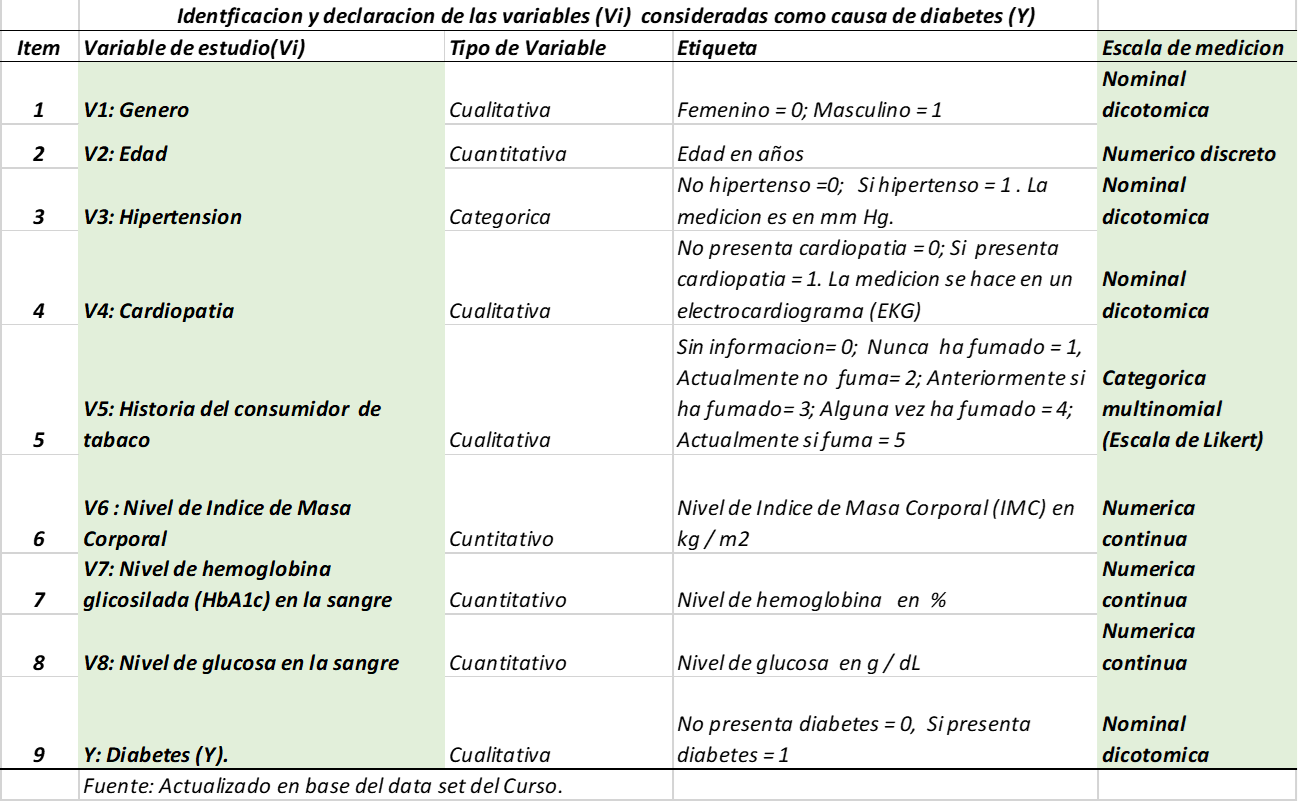
\includegraphics[width=1\linewidth]{tipo_variable} \textbf{Para realizar
el analisis} de acuerdo con el objetivo planteado, filtraremos el
dataset inicial para solo quedarnos con los adultos. \textbf{a) Adultos
jovenes} de 25 años a 44 años \textbf{b) Adultos medios} de 45 añoss a
59 años \textbf{c) Adultos mayores} mayores a 60 años.

El \textbf{primer paso} sera cargar las librerias que permitiran el
analisis descriptivo de los datos

\begin{Shaded}
\begin{Highlighting}[]
\CommentTok{\#1.CARGAR LIBRERIAS PARA EL ANALISIS DESCRIPTIVO}
\FunctionTok{library}\NormalTok{(}\StringTok{"ggplot2"}\NormalTok{)}
\FunctionTok{library}\NormalTok{(}\StringTok{"tibble"}\NormalTok{)}
\FunctionTok{library}\NormalTok{(}\StringTok{"tidyr"}\NormalTok{)}
\FunctionTok{library}\NormalTok{(}\StringTok{"dplyr"}\NormalTok{)}
\FunctionTok{library}\NormalTok{(}\StringTok{"forcats"}\NormalTok{)}
\FunctionTok{library}\NormalTok{(}\StringTok{"purrr"}\NormalTok{)}
\FunctionTok{library}\NormalTok{(}\StringTok{"prismatic"}\NormalTok{)}
\FunctionTok{library}\NormalTok{(}\StringTok{"corrr"}\NormalTok{)}
\FunctionTok{library}\NormalTok{(}\StringTok{"cowplot"}\NormalTok{)}
\FunctionTok{library}\NormalTok{(}\StringTok{"ggforce"}\NormalTok{)}
\FunctionTok{library}\NormalTok{(}\StringTok{"ggrepel"}\NormalTok{)}
\FunctionTok{library}\NormalTok{(}\StringTok{"ggridges"}\NormalTok{)}
\FunctionTok{library}\NormalTok{(}\StringTok{"ggsci"}\NormalTok{)}
\FunctionTok{library}\NormalTok{(}\StringTok{"ggtext"}\NormalTok{)}
\FunctionTok{library}\NormalTok{(}\StringTok{"ggthemes"}\NormalTok{)}
\FunctionTok{library}\NormalTok{(}\StringTok{"summarytools"}\NormalTok{)}
\FunctionTok{library}\NormalTok{(}\StringTok{"grid"}\NormalTok{)}
\FunctionTok{library}\NormalTok{(}\StringTok{"gridExtra"}\NormalTok{)}
\FunctionTok{library}\NormalTok{(}\StringTok{"patchwork"}\NormalTok{)}
\FunctionTok{library}\NormalTok{(}\StringTok{"rcartocolor"}\NormalTok{)}
\FunctionTok{library}\NormalTok{(}\StringTok{"scico"}\NormalTok{)}
\FunctionTok{library}\NormalTok{(}\StringTok{"showtext"}\NormalTok{)}
\FunctionTok{library}\NormalTok{(}\StringTok{"shiny"}\NormalTok{)}
\FunctionTok{library}\NormalTok{(}\StringTok{"plotly"}\NormalTok{)}
\FunctionTok{library}\NormalTok{(}\StringTok{"highcharter"}\NormalTok{)}
\FunctionTok{library}\NormalTok{(}\StringTok{"echarts4r"}\NormalTok{)}
\end{Highlighting}
\end{Shaded}

El \textbf{segundo paso} será establecer el directorio de trabajo y
cargar los datos desde el directorio de trabajo

\begin{Shaded}
\begin{Highlighting}[]
\CommentTok{\#2. Establecer el directorio de trabajo local}
\FunctionTok{getwd}\NormalTok{() }\CommentTok{\#Consultar el directorio de trabajo actual }
\end{Highlighting}
\end{Shaded}

\begin{verbatim}
## [1] "G:/Mi unidad/REPO/Adelmo/AdemoOchoaNolasco.github.io"
\end{verbatim}

\begin{Shaded}
\begin{Highlighting}[]
\FunctionTok{setwd}\NormalTok{(}\StringTok{"G:/Mi unidad/REPO/Adelmo/AdemoOchoaNolasco.github.io"}\NormalTok{)  }\CommentTok{\# Establecer el entorno de trabajo}
\end{Highlighting}
\end{Shaded}

El \textbf{tercer paso} será revisar los tipos de variable con ls
funcion y el calculo de algunos estadistivos univariados

\begin{Shaded}
\begin{Highlighting}[]
\CommentTok{\#3. Cargar datos y sumario de datos}
\NormalTok{data\_diabetes}\OtherTok{\textless{}{-}}\FunctionTok{read.csv}\NormalTok{(}\StringTok{\textquotesingle{}./diabetes\_prediction\_dataset.csv\textquotesingle{}}\NormalTok{, }\AttributeTok{encoding =} \StringTok{\textquotesingle{}UTF{-}8\textquotesingle{}}\NormalTok{, }\AttributeTok{sep =} \StringTok{\textquotesingle{};\textquotesingle{}}\NormalTok{)}
\FunctionTok{head}\NormalTok{(data\_diabetes)}
\end{Highlighting}
\end{Shaded}

\begin{verbatim}
##   gender age hypertension heart_disease smoking_history   bmi HbA1c_level blood_glucose_level diabetes
## 1 Female  80            0             1           never 25.19         6.6                 140        0
## 2 Female  54            0             0         No Info 27.32         6.6                  80        0
## 3   Male  28            0             0           never 27.32         5.7                 158        0
## 4 Female  36            0             0         current 23.45         5.0                 155        0
## 5   Male  76            1             1         current 20.14         4.8                 155        0
## 6 Female  20            0             0           never 27.32         6.6                  85        0
\end{verbatim}

\begin{Shaded}
\begin{Highlighting}[]
\FunctionTok{str}\NormalTok{(data\_diabetes)}
\end{Highlighting}
\end{Shaded}

\begin{verbatim}
## 'data.frame':    100000 obs. of  9 variables:
##  $ gender             : chr  "Female" "Female" "Male" "Female" ...
##  $ age                : num  80 54 28 36 76 20 44 79 42 32 ...
##  $ hypertension       : int  0 0 0 0 1 0 0 0 0 0 ...
##  $ heart_disease      : int  1 0 0 0 1 0 0 0 0 0 ...
##  $ smoking_history    : chr  "never" "No Info" "never" "current" ...
##  $ bmi                : num  25.2 27.3 27.3 23.4 20.1 ...
##  $ HbA1c_level        : num  6.6 6.6 5.7 5 4.8 6.6 6.5 5.7 4.8 5 ...
##  $ blood_glucose_level: int  140 80 158 155 155 85 200 85 145 100 ...
##  $ diabetes           : int  0 0 0 0 0 0 1 0 0 0 ...
\end{verbatim}

\begin{Shaded}
\begin{Highlighting}[]
\FunctionTok{summary}\NormalTok{(data\_diabetes)}
\end{Highlighting}
\end{Shaded}

\begin{verbatim}
##     gender               age         hypertension     heart_disease     smoking_history         bmi         HbA1c_level    blood_glucose_level
##  Length:100000      Min.   : 0.08   Min.   :0.00000   Min.   :0.00000   Length:100000      Min.   :10.01   Min.   :3.500   Min.   : 80.0      
##  Class :character   1st Qu.:24.00   1st Qu.:0.00000   1st Qu.:0.00000   Class :character   1st Qu.:23.63   1st Qu.:4.800   1st Qu.:100.0      
##  Mode  :character   Median :43.00   Median :0.00000   Median :0.00000   Mode  :character   Median :27.32   Median :5.800   Median :140.0      
##                     Mean   :41.89   Mean   :0.07485   Mean   :0.03942                      Mean   :27.32   Mean   :5.528   Mean   :138.1      
##                     3rd Qu.:60.00   3rd Qu.:0.00000   3rd Qu.:0.00000                      3rd Qu.:29.58   3rd Qu.:6.200   3rd Qu.:159.0      
##                     Max.   :80.00   Max.   :1.00000   Max.   :1.00000                      Max.   :95.69   Max.   :9.000   Max.   :300.0      
##     diabetes    
##  Min.   :0.000  
##  1st Qu.:0.000  
##  Median :0.000  
##  Mean   :0.085  
##  3rd Qu.:0.000  
##  Max.   :1.000
\end{verbatim}

\hypertarget{b.-creacion-de-los-grupos-de-adultos---grupos-de-interes}{%
\subsubsection{\texorpdfstring{\textbf{B. CREACION DE LOS GRUPOS DE
ADULTOS - GRUPOS DE
INTERES:}}{B. CREACION DE LOS GRUPOS DE ADULTOS - GRUPOS DE INTERES:}}\label{b.-creacion-de-los-grupos-de-adultos---grupos-de-interes}}

Como \textbf{cuarto paso} será el filtrado por edades, con la finalidad
de quedarnos con los grupos de interés. Una vez clasificado los tipos de
adultos, por edades, se establece la variable TIPO\_ADULTO

\begin{Shaded}
\begin{Highlighting}[]
\CommentTok{\#4. Fitrado {-} creación subset de interés}
\DocumentationTok{\#\# ADULTO JOVEN 25 A 44 años}
\NormalTok{diabetes\_25\_44 }\OtherTok{\textless{}{-}}\NormalTok{ data\_diabetes }\SpecialCharTok{\%\textgreater{}\%} \FunctionTok{filter}\NormalTok{(age }\SpecialCharTok{\textgreater{}=}\DecValTok{25}\NormalTok{) }\SpecialCharTok{\%\textgreater{}\%} \FunctionTok{filter}\NormalTok{(age }\SpecialCharTok{\textless{}=}\DecValTok{44}\NormalTok{) }\SpecialCharTok{\%\textgreater{}\%} \FunctionTok{mutate}\NormalTok{(}\AttributeTok{TIPO\_ADULTO =}\StringTok{"1\_Adulto\_Jovenes"}\NormalTok{)}
\FunctionTok{summary}\NormalTok{(diabetes\_25\_44)}
\end{Highlighting}
\end{Shaded}

\begin{verbatim}
##     gender               age         hypertension     heart_disease      smoking_history         bmi         HbA1c_level    blood_glucose_level
##  Length:26523       Min.   :25.00   Min.   :0.00000   Min.   :0.000000   Length:26523       Min.   :10.08   Min.   :3.500   Min.   : 80.0      
##  Class :character   1st Qu.:30.00   1st Qu.:0.00000   1st Qu.:0.000000   Class :character   1st Qu.:25.39   1st Qu.:4.800   1st Qu.:100.0      
##  Mode  :character   Median :35.00   Median :0.00000   Median :0.000000   Mode  :character   Median :27.32   Median :5.800   Median :140.0      
##                     Mean   :34.68   Mean   :0.03148   Mean   :0.004675                      Mean   :28.71   Mean   :5.449   Mean   :134.9      
##                     3rd Qu.:40.00   3rd Qu.:0.00000   3rd Qu.:0.000000                      3rd Qu.:30.70   3rd Qu.:6.200   3rd Qu.:158.0      
##                     Max.   :44.00   Max.   :1.00000   Max.   :1.000000                      Max.   :91.82   Max.   :9.000   Max.   :300.0      
##     diabetes       TIPO_ADULTO       
##  Min.   :0.00000   Length:26523      
##  1st Qu.:0.00000   Class :character  
##  Median :0.00000   Mode  :character  
##  Mean   :0.03589                     
##  3rd Qu.:0.00000                     
##  Max.   :1.00000
\end{verbatim}

\begin{Shaded}
\begin{Highlighting}[]
\DocumentationTok{\#\# ADULTO MADURO{-}MEDIO 45 a 59 años}
\NormalTok{diabetes\_45\_59 }\OtherTok{\textless{}{-}}\NormalTok{ data\_diabetes }\SpecialCharTok{\%\textgreater{}\%} \FunctionTok{filter}\NormalTok{(age }\SpecialCharTok{\textgreater{}=}\DecValTok{45}\NormalTok{) }\SpecialCharTok{\%\textgreater{}\%} \FunctionTok{filter}\NormalTok{(age }\SpecialCharTok{\textless{}=}\DecValTok{59}\NormalTok{) }\SpecialCharTok{\%\textgreater{}\%} \FunctionTok{mutate}\NormalTok{(}\AttributeTok{TIPO\_ADULTO =}\StringTok{"2\_Adulto\_Medios"}\NormalTok{)}
\FunctionTok{summary}\NormalTok{(diabetes\_45\_59)}
\end{Highlighting}
\end{Shaded}

\begin{verbatim}
##     gender               age         hypertension    heart_disease     smoking_history         bmi         HbA1c_level    blood_glucose_level
##  Length:22537       Min.   :45.00   Min.   :0.0000   Min.   :0.00000   Length:22537       Min.   :10.50   Min.   :3.500   Min.   : 80.0      
##  Class :character   1st Qu.:48.00   1st Qu.:0.0000   1st Qu.:0.00000   Class :character   1st Qu.:26.56   1st Qu.:4.800   1st Qu.:100.0      
##  Mode  :character   Median :52.00   Median :0.0000   Median :0.00000   Mode  :character   Median :27.32   Median :5.800   Median :140.0      
##                     Mean   :51.89   Mean   :0.1002   Mean   :0.03523                      Mean   :29.48   Mean   :5.574   Mean   :139.6      
##                     3rd Qu.:56.00   3rd Qu.:0.0000   3rd Qu.:0.00000                      3rd Qu.:31.92   3rd Qu.:6.200   3rd Qu.:159.0      
##                     Max.   :59.00   Max.   :1.0000   Max.   :1.00000                      Max.   :88.72   Max.   :9.000   Max.   :300.0      
##     diabetes      TIPO_ADULTO       
##  Min.   :0.0000   Length:22537      
##  1st Qu.:0.0000   Class :character  
##  Median :0.0000   Mode  :character  
##  Mean   :0.1092                     
##  3rd Qu.:0.0000                     
##  Max.   :1.0000
\end{verbatim}

\begin{Shaded}
\begin{Highlighting}[]
\DocumentationTok{\#\# ADULTO MAYOR 60 a más}
\NormalTok{diabetes\_60 }\OtherTok{\textless{}{-}}\NormalTok{ data\_diabetes }\SpecialCharTok{\%\textgreater{}\%} \FunctionTok{filter}\NormalTok{(age }\SpecialCharTok{\textgreater{}=}\DecValTok{60}\NormalTok{) }\SpecialCharTok{\%\textgreater{}\%} \FunctionTok{mutate}\NormalTok{(}\AttributeTok{TIPO\_ADULTO =}\StringTok{"3\_Adulto\_Mayores"}\NormalTok{)}
\FunctionTok{summary}\NormalTok{(diabetes\_60)}
\end{Highlighting}
\end{Shaded}

\begin{verbatim}
##     gender               age         hypertension    heart_disease    smoking_history         bmi         HbA1c_level    blood_glucose_level
##  Length:25055       Min.   :60.00   Min.   :0.0000   Min.   :0.0000   Length:25055       Min.   :10.01   Min.   :3.500   Min.   : 80.0      
##  Class :character   1st Qu.:64.00   1st Qu.:0.0000   1st Qu.:0.0000   Class :character   1st Qu.:26.04   1st Qu.:4.800   1st Qu.:126.0      
##  Mode  :character   Median :70.00   Median :0.0000   Median :0.0000   Mode  :character   Median :27.32   Median :5.800   Median :145.0      
##                     Mean   :70.76   Mean   :0.1737   Mean   :0.1203                      Mean   :28.55   Mean   :5.694   Mean   :145.2      
##                     3rd Qu.:78.00   3rd Qu.:0.0000   3rd Qu.:0.0000                      3rd Qu.:30.47   3rd Qu.:6.500   3rd Qu.:159.0      
##                     Max.   :80.00   Max.   :1.0000   Max.   :1.0000                      Max.   :88.76   Max.   :9.000   Max.   :300.0      
##     diabetes      TIPO_ADULTO       
##  Min.   :0.0000   Length:25055      
##  1st Qu.:0.0000   Class :character  
##  Median :0.0000   Mode  :character  
##  Mean   :0.1968                     
##  3rd Qu.:0.0000                     
##  Max.   :1.0000
\end{verbatim}

\hypertarget{c.-estadistica-descriptiva---grupos-de-interes}{%
\subsubsection{\texorpdfstring{\textbf{C. ESTADISTICA DESCRIPTIVA -
GRUPOS DE
INTERES:}}{C. ESTADISTICA DESCRIPTIVA - GRUPOS DE INTERES:}}\label{c.-estadistica-descriptiva---grupos-de-interes}}

\textbf{Finalmente} una vez seleccionado los grupos de interes, se tiene
el siguiente dataset actualizado diabetes\_Grupoadultos Se revisa las
variables

\begin{Shaded}
\begin{Highlighting}[]
\NormalTok{diabetes\_Grupoadultos }\OtherTok{\textless{}{-}} \FunctionTok{bind\_rows}\NormalTok{(diabetes\_25\_44,diabetes\_45\_59,diabetes\_60)}
\FunctionTok{str}\NormalTok{(diabetes\_Grupoadultos)}
\end{Highlighting}
\end{Shaded}

\begin{verbatim}
## 'data.frame':    74115 obs. of  10 variables:
##  $ gender             : chr  "Male" "Female" "Female" "Male" ...
##  $ age                : num  28 36 44 42 32 42 42 37 40 30 ...
##  $ hypertension       : int  0 0 0 0 0 0 0 0 0 0 ...
##  $ heart_disease      : int  0 0 0 0 0 0 0 0 0 0 ...
##  $ smoking_history    : chr  "never" "current" "never" "never" ...
##  $ bmi                : num  27.3 23.4 19.3 33.6 27.3 ...
##  $ HbA1c_level        : num  5.7 5 6.5 4.8 5 5.7 5.7 3.5 6 6.1 ...
##  $ blood_glucose_level: int  158 155 200 145 100 158 80 159 90 126 ...
##  $ diabetes           : int  0 0 1 0 0 0 0 0 0 0 ...
##  $ TIPO_ADULTO        : chr  "1_Adulto_Jovenes" "1_Adulto_Jovenes" "1_Adulto_Jovenes" "1_Adulto_Jovenes" ...
\end{verbatim}

Se realiza la tabla de frecuencias

\begin{Shaded}
\begin{Highlighting}[]
\FunctionTok{freq}\NormalTok{(diabetes\_Grupoadultos}\SpecialCharTok{$}\NormalTok{TIPO\_ADULTO , }\AttributeTok{style =} \StringTok{"rmarkdown"}\NormalTok{, }\AttributeTok{justify =} \StringTok{"center"}\NormalTok{, }\AttributeTok{headings =} \ConstantTok{TRUE}\NormalTok{, }\AttributeTok{report.nas =} \ConstantTok{FALSE}\NormalTok{)}
\end{Highlighting}
\end{Shaded}

\begin{verbatim}
## setting plain.ascii to FALSE
\end{verbatim}

\begin{verbatim}
## ### Frequencies  
## 
## |        &nbsp;        | Freq  |   %    | % Cum. |
## |:--------------------:|:-----:|:------:|:------:|
## | **1_Adulto_Jovenes** | 26523 | 35.79  | 35.79  |
## | **2_Adulto_Medios**  | 22537 | 30.41  | 66.19  |
## | **3_Adulto_Mayores** | 25055 | 33.81  | 100.00 |
## |      **Total**       | 74115 | 100.00 | 100.00 |
\end{verbatim}

\begin{Shaded}
\begin{Highlighting}[]
\NormalTok{tabla\_frecuencia }\OtherTok{\textless{}{-}} \FunctionTok{table}\NormalTok{(diabetes\_Grupoadultos}\SpecialCharTok{$}\NormalTok{TIPO\_ADULTO, diabetes\_Grupoadultos}\SpecialCharTok{$}\NormalTok{gender, diabetes\_Grupoadultos}\SpecialCharTok{$}\NormalTok{diabetes)}
                               
\CommentTok{\# Convertir la tabla de frecuencia en un marco de datos para mejor visualización}
\NormalTok{df\_tabla\_frecuencia }\OtherTok{\textless{}{-}} \FunctionTok{as.data.frame}\NormalTok{(tabla\_frecuencia)}
\FunctionTok{colnames}\NormalTok{(df\_tabla\_frecuencia) }\OtherTok{\textless{}{-}} \FunctionTok{c}\NormalTok{(}\StringTok{"Tipo de Adulto"}\NormalTok{,}\StringTok{"Género"}\NormalTok{,}\StringTok{"Diabetes Si (1) {-} No (0)"}\NormalTok{,}\StringTok{"Freq"}\NormalTok{)}

\CommentTok{\# Imprimir la tabla de frecuencias por tipo de adulto y genero}
\NormalTok{knitr}\SpecialCharTok{::}\FunctionTok{kable}\NormalTok{(df\_tabla\_frecuencia, }\AttributeTok{caption =} \StringTok{"Frecuencia de combinaciones de Tipo de adulto , género y presencia de diabetes"}\NormalTok{)}
\end{Highlighting}
\end{Shaded}

\begin{longtable}[]{@{}lllr@{}}
\caption{Frecuencia de combinaciones de Tipo de adulto , género y
presencia de diabetes}\tabularnewline
\toprule\noalign{}
Tipo de Adulto & Género & Diabetes Si (1) - No (0) & Freq \\
\midrule\noalign{}
\endfirsthead
\toprule\noalign{}
Tipo de Adulto & Género & Diabetes Si (1) - No (0) & Freq \\
\midrule\noalign{}
\endhead
\bottomrule\noalign{}
\endlastfoot
1\_Adulto\_Jovenes & Female & 0 & 16177 \\
2\_Adulto\_Medios & Female & 0 & 12030 \\
3\_Adulto\_Mayores & Female & 0 & 11976 \\
1\_Adulto\_Jovenes & Male & 0 & 9391 \\
2\_Adulto\_Medios & Male & 0 & 8040 \\
3\_Adulto\_Mayores & Male & 0 & 8147 \\
1\_Adulto\_Jovenes & Other & 0 & 3 \\
2\_Adulto\_Medios & Other & 0 & 6 \\
3\_Adulto\_Mayores & Other & 0 & 0 \\
1\_Adulto\_Jovenes & Female & 1 & 535 \\
2\_Adulto\_Medios & Female & 1 & 1239 \\
3\_Adulto\_Mayores & Female & 1 & 2604 \\
1\_Adulto\_Jovenes & Male & 1 & 417 \\
2\_Adulto\_Medios & Male & 1 & 1222 \\
3\_Adulto\_Mayores & Male & 1 & 2328 \\
1\_Adulto\_Jovenes & Other & 1 & 0 \\
2\_Adulto\_Medios & Other & 1 & 0 \\
3\_Adulto\_Mayores & Other & 1 & 0 \\
\end{longtable}

\textbf{Relación entre Glucosa en Sangre y BMI} en Grupos de Adultos

\begin{Shaded}
\begin{Highlighting}[]
\FunctionTok{library}\NormalTok{(ggplot2)}
\FunctionTok{ggplot}\NormalTok{(diabetes\_Grupoadultos, }\FunctionTok{aes}\NormalTok{(}\AttributeTok{x =}\NormalTok{ blood\_glucose\_level, }\AttributeTok{y =}\NormalTok{ bmi)) }\SpecialCharTok{+}
  \FunctionTok{geom\_point}\NormalTok{(}\AttributeTok{color =} \StringTok{"orangered"}\NormalTok{, }\AttributeTok{alpha =}\NormalTok{ .}\DecValTok{2}\NormalTok{) }\SpecialCharTok{+}
  \FunctionTok{theme}\NormalTok{(}\AttributeTok{axis.text.x =} \FunctionTok{element\_text}\NormalTok{(}\AttributeTok{angle =} \DecValTok{45}\NormalTok{, }\AttributeTok{vjust =} \DecValTok{1}\NormalTok{, }\AttributeTok{hjust =} \DecValTok{1}\NormalTok{)) }\SpecialCharTok{+}
  \FunctionTok{labs}\NormalTok{(}\AttributeTok{x =} \StringTok{"blood\_glucose\_level mg/dl"}\NormalTok{, }\AttributeTok{y =} \StringTok{"bmi (kg/m2)"}\NormalTok{, }\AttributeTok{title =} \StringTok{"Relación entre Glucosa en Sangre y BMI en Grupos de Adultos}\SpecialCharTok{\textbackslash{}n}\StringTok{sin Diabetes (0) y con Diabetes(1)"}\NormalTok{) }\SpecialCharTok{+}
  \FunctionTok{facet\_grid}\NormalTok{(TIPO\_ADULTO }\SpecialCharTok{\textasciitilde{}}\NormalTok{ diabetes)}
\end{Highlighting}
\end{Shaded}

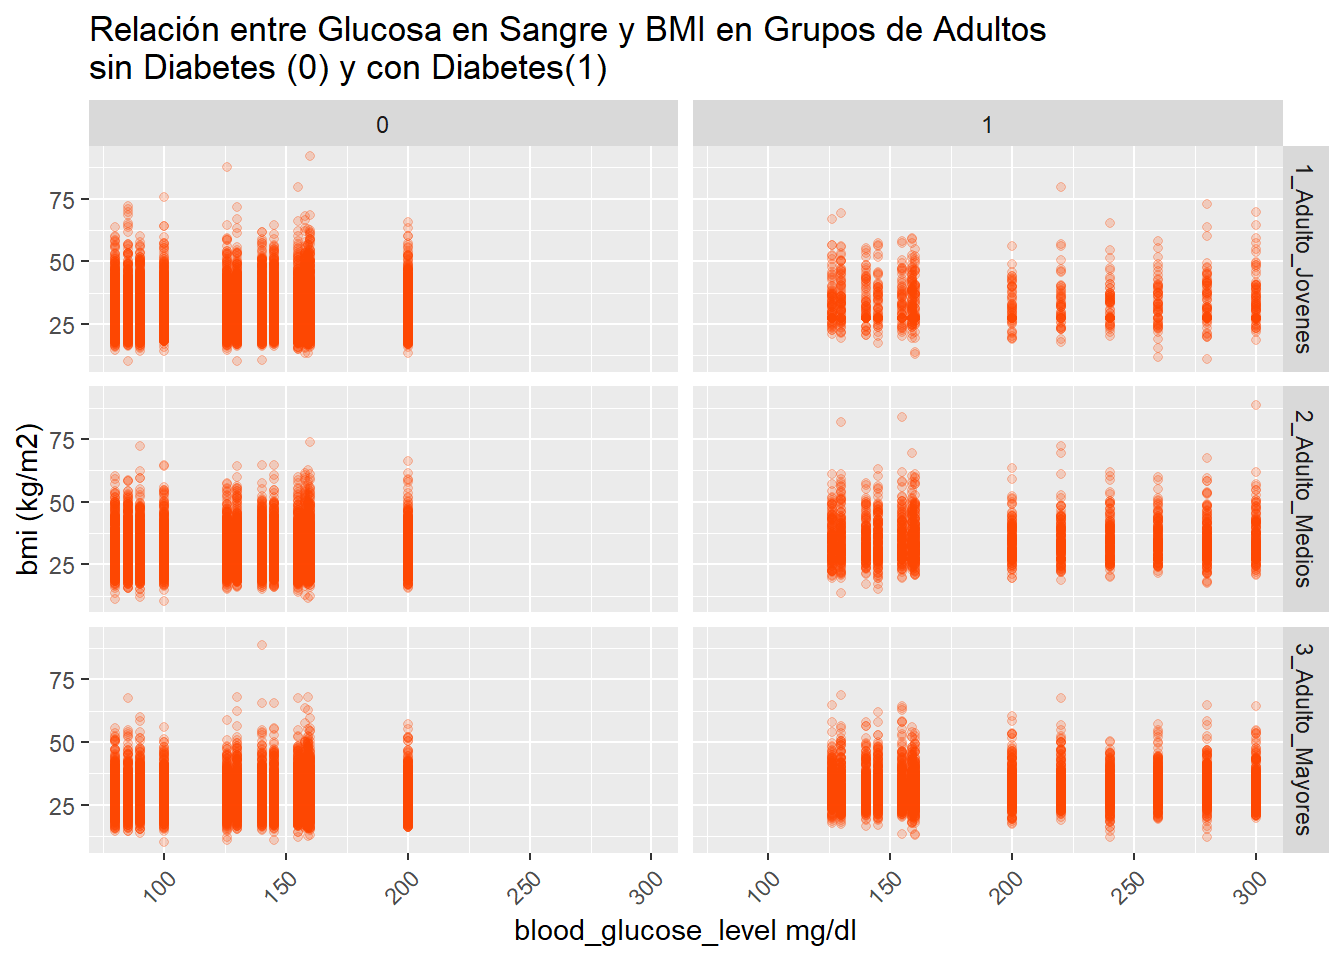
\includegraphics{Variables_files/figure-latex/unnamed-chunk-10-1.pdf}

\begin{Shaded}
\begin{Highlighting}[]
\NormalTok{g }\OtherTok{\textless{}{-}}
  \FunctionTok{ggplot}\NormalTok{(diabetes\_Grupoadultos, }\FunctionTok{aes}\NormalTok{(}\AttributeTok{x =}\NormalTok{ TIPO\_ADULTO, }\AttributeTok{y =}\NormalTok{ HbA1c\_level,}
                   \AttributeTok{color =}\NormalTok{ TIPO\_ADULTO)) }\SpecialCharTok{+}
    \FunctionTok{labs}\NormalTok{(}\AttributeTok{x =} \StringTok{"TIPO\_ADULTO"}\NormalTok{, }\AttributeTok{y =} \StringTok{"HbA1c\_level"}\NormalTok{) }\SpecialCharTok{+}
    \FunctionTok{scale\_color\_brewer}\NormalTok{(}\AttributeTok{palette =} \StringTok{"Dark2"}\NormalTok{, }\AttributeTok{guide =} \StringTok{"none"}\NormalTok{)}

\NormalTok{g }\SpecialCharTok{+} \FunctionTok{geom\_boxplot}\NormalTok{() }\SpecialCharTok{+} \FunctionTok{facet\_wrap}\NormalTok{(}\SpecialCharTok{\textasciitilde{}}\NormalTok{ diabetes)}
\end{Highlighting}
\end{Shaded}

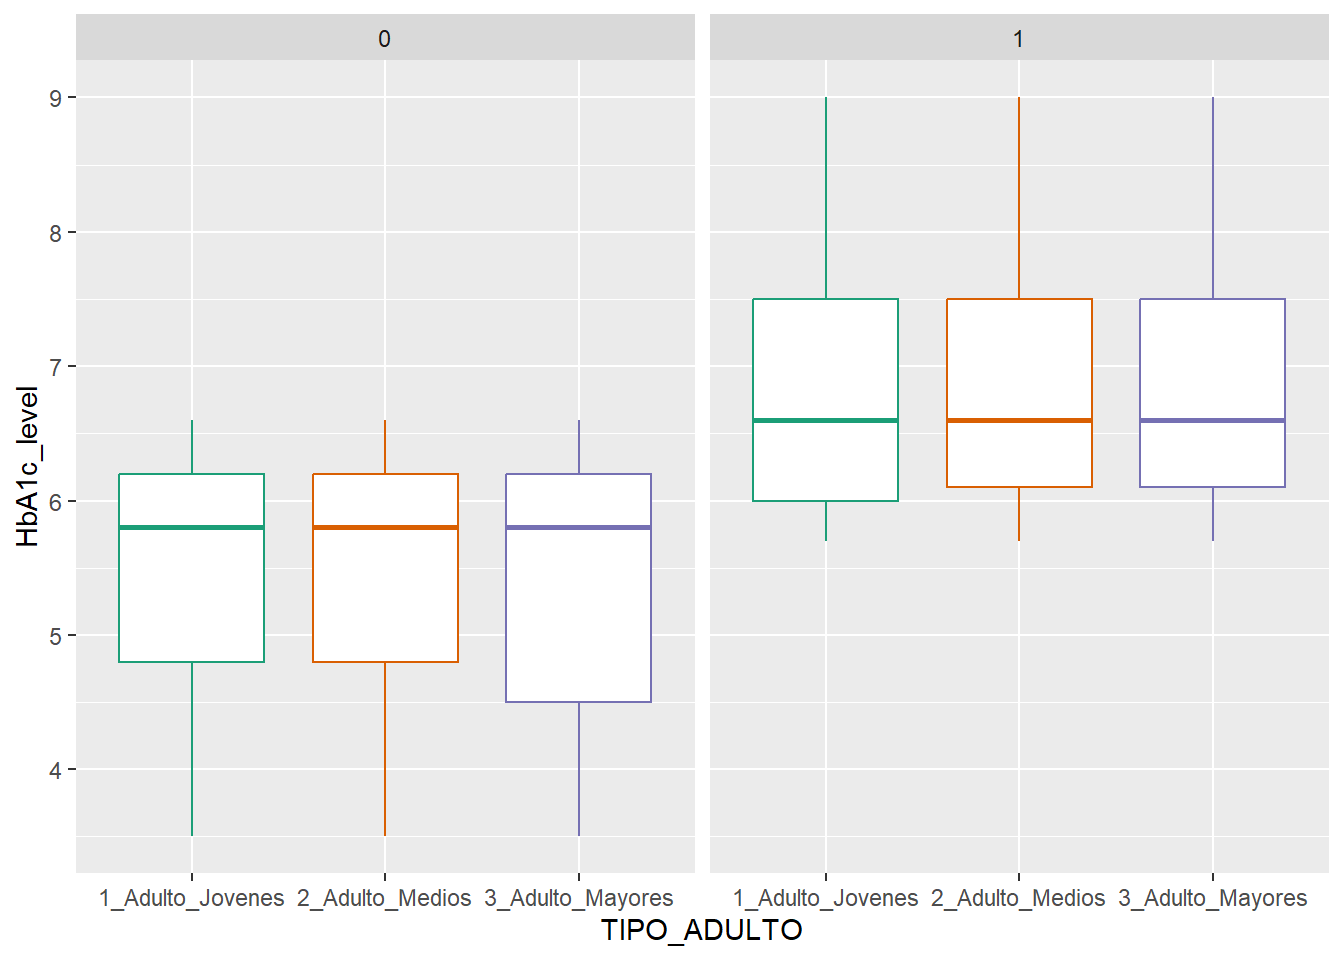
\includegraphics{Variables_files/figure-latex/unnamed-chunk-11-1.pdf}

\hypertarget{d.-tabla-de-estaduxedsticos-univariados---adultos-jovenes}{%
\subsubsection{\texorpdfstring{\textbf{D. Tabla de estadísticos
univariados - Adultos
jovenes:}}{D. Tabla de estadísticos univariados - Adultos jovenes:}}\label{d.-tabla-de-estaduxedsticos-univariados---adultos-jovenes}}

Se calcula los estadisticos univariados para el grupo de adultos jovenes

\begin{Shaded}
\begin{Highlighting}[]
\FunctionTok{descr}\NormalTok{(diabetes\_25\_44}\SpecialCharTok{$}\NormalTok{bmi, }\AttributeTok{transpose =} \ConstantTok{TRUE}\NormalTok{, }
      \AttributeTok{stats =} \FunctionTok{c}\NormalTok{(}\StringTok{"N.Valid"}\NormalTok{, }\StringTok{"min"}\NormalTok{,}\StringTok{"q1"}\NormalTok{,}\StringTok{"med"}\NormalTok{,}\StringTok{"mean"}\NormalTok{,}\StringTok{"sd"}\NormalTok{,}\StringTok{"q3"}\NormalTok{,}\StringTok{"max"}\NormalTok{,}\StringTok{"iqr"}\NormalTok{),}
      \AttributeTok{style =} \StringTok{"rmarkdown"}\NormalTok{, }\AttributeTok{justify =} \StringTok{"center"}\NormalTok{, }\AttributeTok{headings =}\NormalTok{ T)}
\end{Highlighting}
\end{Shaded}

\begin{verbatim}
## ### Descriptive Statistics  
## #### value  
## **N:** 26523  
## 
## |  &nbsp;   | N.Valid  |  Min  |  Q1   | Median | Mean  | Std.Dev |  Q3   |  Max  | IQR  |
## |:---------:|:--------:|:-----:|:-----:|:------:|:-----:|:-------:|:-----:|:-----:|:----:|
## | **value** | 26523.00 | 10.08 | 25.39 | 27.32  | 28.71 |  6.40   | 30.70 | 91.82 | 5.31 |
\end{verbatim}

\begin{Shaded}
\begin{Highlighting}[]
\FunctionTok{descr}\NormalTok{(diabetes\_25\_44}\SpecialCharTok{$}\NormalTok{HbA1c\_level, }\AttributeTok{transpose =} \ConstantTok{TRUE}\NormalTok{, }
      \AttributeTok{stats =} \FunctionTok{c}\NormalTok{(}\StringTok{"N.Valid"}\NormalTok{, }\StringTok{"min"}\NormalTok{,}\StringTok{"q1"}\NormalTok{,}\StringTok{"med"}\NormalTok{,}\StringTok{"mean"}\NormalTok{,}\StringTok{"sd"}\NormalTok{,}\StringTok{"q3"}\NormalTok{,}\StringTok{"max"}\NormalTok{,}\StringTok{"iqr"}\NormalTok{),}
      \AttributeTok{style =} \StringTok{"rmarkdown"}\NormalTok{, }\AttributeTok{justify =} \StringTok{"center"}\NormalTok{, }\AttributeTok{headings =}\NormalTok{ T)}
\end{Highlighting}
\end{Shaded}

\begin{verbatim}
## ### Descriptive Statistics  
## #### value  
## **N:** 26523  
## 
## |  &nbsp;   | N.Valid  | Min  |  Q1  | Median | Mean | Std.Dev |  Q3  | Max  | IQR  |
## |:---------:|:--------:|:----:|:----:|:------:|:----:|:-------:|:----:|:----:|:----:|
## | **value** | 26523.00 | 3.50 | 4.80 |  5.80  | 5.45 |  1.02   | 6.20 | 9.00 | 1.40 |
\end{verbatim}

\begin{Shaded}
\begin{Highlighting}[]
\FunctionTok{descr}\NormalTok{(diabetes\_25\_44}\SpecialCharTok{$}\NormalTok{blood\_glucose\_level, }\AttributeTok{transpose =} \ConstantTok{TRUE}\NormalTok{, }
      \AttributeTok{stats =} \FunctionTok{c}\NormalTok{(}\StringTok{"N.Valid"}\NormalTok{, }\StringTok{"min"}\NormalTok{,}\StringTok{"q1"}\NormalTok{,}\StringTok{"med"}\NormalTok{,}\StringTok{"mean"}\NormalTok{,}\StringTok{"sd"}\NormalTok{,}\StringTok{"q3"}\NormalTok{,}\StringTok{"max"}\NormalTok{,}\StringTok{"iqr"}\NormalTok{),}
      \AttributeTok{style =} \StringTok{"rmarkdown"}\NormalTok{, }\AttributeTok{justify =} \StringTok{"center"}\NormalTok{, }\AttributeTok{headings =}\NormalTok{ T)}
\end{Highlighting}
\end{Shaded}

\begin{verbatim}
## ### Descriptive Statistics  
## #### value  
## **N:** 26523  
## 
## |  &nbsp;   | N.Valid  |  Min  |   Q1   | Median |  Mean  | Std.Dev |   Q3   |  Max   |  IQR  |
## |:---------:|:--------:|:-----:|:------:|:------:|:------:|:-------:|:------:|:------:|:-----:|
## | **value** | 26523.00 | 80.00 | 100.00 | 140.00 | 134.87 |  37.27  | 158.00 | 300.00 | 58.00 |
\end{verbatim}

\hypertarget{e.-tabla-de-estaduxedsticos-univariados---adultos-medios}{%
\subsubsection{\texorpdfstring{\textbf{E. Tabla de estadísticos
univariados - Adultos
medios:}}{E. Tabla de estadísticos univariados - Adultos medios:}}\label{e.-tabla-de-estaduxedsticos-univariados---adultos-medios}}

Se calcula los estadisticos univariados para el grupo de adultos medios

\begin{Shaded}
\begin{Highlighting}[]
\FunctionTok{descr}\NormalTok{(diabetes\_45\_59}\SpecialCharTok{$}\NormalTok{bmi, }\AttributeTok{transpose =} \ConstantTok{TRUE}\NormalTok{, }
      \AttributeTok{stats =} \FunctionTok{c}\NormalTok{(}\StringTok{"N.Valid"}\NormalTok{, }\StringTok{"min"}\NormalTok{,}\StringTok{"q1"}\NormalTok{,}\StringTok{"med"}\NormalTok{,}\StringTok{"mean"}\NormalTok{,}\StringTok{"sd"}\NormalTok{,}\StringTok{"q3"}\NormalTok{,}\StringTok{"max"}\NormalTok{,}\StringTok{"iqr"}\NormalTok{),}
      \AttributeTok{style =} \StringTok{"rmarkdown"}\NormalTok{, }\AttributeTok{justify =} \StringTok{"center"}\NormalTok{, }\AttributeTok{headings =}\NormalTok{ T)}
\end{Highlighting}
\end{Shaded}

\begin{verbatim}
## ### Descriptive Statistics  
## #### value  
## **N:** 22537  
## 
## |  &nbsp;   | N.Valid  |  Min  |  Q1   | Median | Mean  | Std.Dev |  Q3   |  Max  | IQR  |
## |:---------:|:--------:|:-----:|:-----:|:------:|:-----:|:-------:|:-----:|:-----:|:----:|
## | **value** | 22537.00 | 10.50 | 26.56 | 27.32  | 29.48 |  6.28   | 31.92 | 88.72 | 5.36 |
\end{verbatim}

\begin{Shaded}
\begin{Highlighting}[]
\FunctionTok{descr}\NormalTok{(diabetes\_45\_59}\SpecialCharTok{$}\NormalTok{HbA1c\_level, }\AttributeTok{transpose =} \ConstantTok{TRUE}\NormalTok{, }
      \AttributeTok{stats =} \FunctionTok{c}\NormalTok{(}\StringTok{"N.Valid"}\NormalTok{, }\StringTok{"min"}\NormalTok{,}\StringTok{"q1"}\NormalTok{,}\StringTok{"med"}\NormalTok{,}\StringTok{"mean"}\NormalTok{,}\StringTok{"sd"}\NormalTok{,}\StringTok{"q3"}\NormalTok{,}\StringTok{"max"}\NormalTok{,}\StringTok{"iqr"}\NormalTok{),}
      \AttributeTok{style =} \StringTok{"rmarkdown"}\NormalTok{, }\AttributeTok{justify =} \StringTok{"center"}\NormalTok{, }\AttributeTok{headings =}\NormalTok{ T)}
\end{Highlighting}
\end{Shaded}

\begin{verbatim}
## ### Descriptive Statistics  
## #### value  
## **N:** 22537  
## 
## |  &nbsp;   | N.Valid  | Min  |  Q1  | Median | Mean | Std.Dev |  Q3  | Max  | IQR  |
## |:---------:|:--------:|:----:|:----:|:------:|:----:|:-------:|:----:|:----:|:----:|
## | **value** | 22537.00 | 3.50 | 4.80 |  5.80  | 5.57 |  1.09   | 6.20 | 9.00 | 1.40 |
\end{verbatim}

\begin{Shaded}
\begin{Highlighting}[]
\FunctionTok{descr}\NormalTok{(diabetes\_45\_59}\SpecialCharTok{$}\NormalTok{blood\_glucose\_level, }\AttributeTok{transpose =} \ConstantTok{TRUE}\NormalTok{, }
      \AttributeTok{stats =} \FunctionTok{c}\NormalTok{(}\StringTok{"N.Valid"}\NormalTok{, }\StringTok{"min"}\NormalTok{,}\StringTok{"q1"}\NormalTok{,}\StringTok{"med"}\NormalTok{,}\StringTok{"mean"}\NormalTok{,}\StringTok{"sd"}\NormalTok{,}\StringTok{"q3"}\NormalTok{,}\StringTok{"max"}\NormalTok{,}\StringTok{"iqr"}\NormalTok{),}
      \AttributeTok{style =} \StringTok{"rmarkdown"}\NormalTok{, }\AttributeTok{justify =} \StringTok{"center"}\NormalTok{, }\AttributeTok{headings =}\NormalTok{ T)}
\end{Highlighting}
\end{Shaded}

\begin{verbatim}
## ### Descriptive Statistics  
## #### value  
## **N:** 22537  
## 
## |  &nbsp;   | N.Valid  |  Min  |   Q1   | Median |  Mean  | Std.Dev |   Q3   |  Max   |  IQR  |
## |:---------:|:--------:|:-----:|:------:|:------:|:------:|:-------:|:------:|:------:|:-----:|
## | **value** | 22537.00 | 80.00 | 100.00 | 140.00 | 139.62 |  41.95  | 159.00 | 300.00 | 59.00 |
\end{verbatim}

\hypertarget{f.-tabla-de-estaduxedsticos-univariados---adultos-mayores}{%
\subsubsection{\texorpdfstring{\textbf{F. Tabla de estadísticos
univariados - Adultos
mayores:}}{F. Tabla de estadísticos univariados - Adultos mayores:}}\label{f.-tabla-de-estaduxedsticos-univariados---adultos-mayores}}

Se calcula los estadisticos univariados para el grupo de adultos mayores

\begin{Shaded}
\begin{Highlighting}[]
\FunctionTok{descr}\NormalTok{(diabetes\_60}\SpecialCharTok{$}\NormalTok{bmi, }\AttributeTok{transpose =} \ConstantTok{TRUE}\NormalTok{, }
      \AttributeTok{stats =} \FunctionTok{c}\NormalTok{(}\StringTok{"N.Valid"}\NormalTok{, }\StringTok{"min"}\NormalTok{,}\StringTok{"q1"}\NormalTok{,}\StringTok{"med"}\NormalTok{,}\StringTok{"mean"}\NormalTok{,}\StringTok{"sd"}\NormalTok{,}\StringTok{"q3"}\NormalTok{,}\StringTok{"max"}\NormalTok{,}\StringTok{"iqr"}\NormalTok{),}
      \AttributeTok{style =} \StringTok{"rmarkdown"}\NormalTok{, }\AttributeTok{justify =} \StringTok{"center"}\NormalTok{, }\AttributeTok{headings =}\NormalTok{ T)}
\end{Highlighting}
\end{Shaded}

\begin{verbatim}
## ### Descriptive Statistics  
## #### value  
## **N:** 25055  
## 
## |  &nbsp;   | N.Valid  |  Min  |  Q1   | Median | Mean  | Std.Dev |  Q3   |  Max  | IQR  |
## |:---------:|:--------:|:-----:|:-----:|:------:|:-----:|:-------:|:-----:|:-----:|:----:|
## | **value** | 25055.00 | 10.01 | 26.04 | 27.32  | 28.55 |  5.46   | 30.47 | 88.76 | 4.43 |
\end{verbatim}

\begin{Shaded}
\begin{Highlighting}[]
\FunctionTok{descr}\NormalTok{(diabetes\_60}\SpecialCharTok{$}\NormalTok{HbA1c\_level, }\AttributeTok{transpose =} \ConstantTok{TRUE}\NormalTok{, }
      \AttributeTok{stats =} \FunctionTok{c}\NormalTok{(}\StringTok{"N.Valid"}\NormalTok{, }\StringTok{"min"}\NormalTok{,}\StringTok{"q1"}\NormalTok{,}\StringTok{"med"}\NormalTok{,}\StringTok{"mean"}\NormalTok{,}\StringTok{"sd"}\NormalTok{,}\StringTok{"q3"}\NormalTok{,}\StringTok{"max"}\NormalTok{,}\StringTok{"iqr"}\NormalTok{),}
      \AttributeTok{style =} \StringTok{"rmarkdown"}\NormalTok{, }\AttributeTok{justify =} \StringTok{"center"}\NormalTok{, }\AttributeTok{headings =}\NormalTok{ T)}
\end{Highlighting}
\end{Shaded}

\begin{verbatim}
## ### Descriptive Statistics  
## #### value  
## **N:** 25055  
## 
## |  &nbsp;   | N.Valid  | Min  |  Q1  | Median | Mean | Std.Dev |  Q3  | Max  | IQR  |
## |:---------:|:--------:|:----:|:----:|:------:|:----:|:-------:|:----:|:----:|:----:|
## | **value** | 25055.00 | 3.50 | 4.80 |  5.80  | 5.69 |  1.17   | 6.50 | 9.00 | 1.70 |
\end{verbatim}

\begin{Shaded}
\begin{Highlighting}[]
\FunctionTok{descr}\NormalTok{(diabetes\_60}\SpecialCharTok{$}\NormalTok{blood\_glucose\_level, }\AttributeTok{transpose =} \ConstantTok{TRUE}\NormalTok{, }
      \AttributeTok{stats =} \FunctionTok{c}\NormalTok{(}\StringTok{"N.Valid"}\NormalTok{, }\StringTok{"min"}\NormalTok{,}\StringTok{"q1"}\NormalTok{,}\StringTok{"med"}\NormalTok{,}\StringTok{"mean"}\NormalTok{,}\StringTok{"sd"}\NormalTok{,}\StringTok{"q3"}\NormalTok{,}\StringTok{"max"}\NormalTok{,}\StringTok{"iqr"}\NormalTok{),}
      \AttributeTok{style =} \StringTok{"rmarkdown"}\NormalTok{, }\AttributeTok{justify =} \StringTok{"center"}\NormalTok{, }\AttributeTok{headings =}\NormalTok{ T)}
\end{Highlighting}
\end{Shaded}

\begin{verbatim}
## ### Descriptive Statistics  
## #### value  
## **N:** 25055  
## 
## |  &nbsp;   | N.Valid  |  Min  |   Q1   | Median |  Mean  | Std.Dev |   Q3   |  Max   |  IQR  |
## |:---------:|:--------:|:-----:|:------:|:------:|:------:|:-------:|:------:|:------:|:-----:|
## | **value** | 25055.00 | 80.00 | 126.00 | 145.00 | 145.18 |  47.21  | 159.00 | 300.00 | 33.00 |
\end{verbatim}

\hypertarget{resumen-del-grupo-de-personas-con-diabetes}{%
\subsubsection{Resumen del grupo de Personas con
Diabetes}\label{resumen-del-grupo-de-personas-con-diabetes}}

\begin{Shaded}
\begin{Highlighting}[]
\NormalTok{diabetes\_Grupoadultos\_SI }\OtherTok{\textless{}{-}}\NormalTok{diabetes\_Grupoadultos }\SpecialCharTok{\%\textgreater{}\%} \FunctionTok{filter}\NormalTok{(diabetes }\SpecialCharTok{==}\StringTok{"1"}\NormalTok{) }
\FunctionTok{summary}\NormalTok{(diabetes\_Grupoadultos\_SI)}
\end{Highlighting}
\end{Shaded}

\begin{verbatim}
##     gender               age         hypertension    heart_disease    smoking_history         bmi         HbA1c_level    blood_glucose_level
##  Length:8345        Min.   :25.00   Min.   :0.0000   Min.   :0.0000   Length:8345        Min.   :10.98   Min.   :5.700   Min.   :126.0      
##  Class :character   1st Qu.:53.00   1st Qu.:0.0000   1st Qu.:0.0000   Class :character   1st Qu.:27.32   1st Qu.:6.100   1st Qu.:145.0      
##  Mode  :character   Median :63.00   Median :0.0000   Median :0.0000   Mode  :character   Median :30.09   Median :6.600   Median :160.0      
##                     Mean   :61.78   Mean   :0.2502   Mean   :0.1517                      Mean   :32.12   Mean   :6.934   Mean   :194.1      
##                     3rd Qu.:73.00   3rd Qu.:1.0000   3rd Qu.:0.0000                      3rd Qu.:36.03   3rd Qu.:7.500   3rd Qu.:240.0      
##                     Max.   :80.00   Max.   :1.0000   Max.   :1.0000                      Max.   :88.72   Max.   :9.000   Max.   :300.0      
##     diabetes TIPO_ADULTO       
##  Min.   :1   Length:8345       
##  1st Qu.:1   Class :character  
##  Median :1   Mode  :character  
##  Mean   :1                     
##  3rd Qu.:1                     
##  Max.   :1
\end{verbatim}

\hypertarget{g.-analizando-la-variable-bmi---body-mass-index}{%
\subsubsection{\texorpdfstring{\textbf{G. Analizando la variable bmi -
Body mass
index:}}{G. Analizando la variable bmi - Body mass index:}}\label{g.-analizando-la-variable-bmi---body-mass-index}}

\textbf{Comentario} Las medianas de los personas con diabetes son
mayores a las que no tienen la enfermedad . Para todos los grupos de
adultos.

\begin{Shaded}
\begin{Highlighting}[]
\DocumentationTok{\#\# Analizando la variable  bmi  {-} Body mass index }
\CommentTok{\# Boxplot.}
\NormalTok{g }\OtherTok{\textless{}{-}}
  \FunctionTok{ggplot}\NormalTok{(diabetes\_Grupoadultos, }\FunctionTok{aes}\NormalTok{(}\AttributeTok{x =}\NormalTok{ TIPO\_ADULTO, }\AttributeTok{y =}\NormalTok{ bmi,}
                   \AttributeTok{color =}\NormalTok{ TIPO\_ADULTO)) }\SpecialCharTok{+}
    \FunctionTok{labs}\NormalTok{(}\AttributeTok{x =} \StringTok{"TIPO\_ADULTO"}\NormalTok{, }\AttributeTok{y =} \StringTok{"bmi (kg/m2)"}\NormalTok{, }\AttributeTok{title =} \StringTok{"Diagrama de cajas del BMI en Grupos de Adultos}\SpecialCharTok{\textbackslash{}n}\StringTok{sin Diabetes (0) y con Diabetes(1)"}\NormalTok{) }\SpecialCharTok{+}
    \FunctionTok{scale\_color\_brewer}\NormalTok{(}\AttributeTok{palette =} \StringTok{"Dark2"}\NormalTok{, }\AttributeTok{guide =} \StringTok{"none"}\NormalTok{)}

\NormalTok{g }\SpecialCharTok{+} \FunctionTok{geom\_boxplot}\NormalTok{() }\SpecialCharTok{+}    \FunctionTok{stat\_boxplot}\NormalTok{(}\AttributeTok{geom =} \StringTok{"errorbar"}\NormalTok{,}
               \AttributeTok{width =} \FloatTok{0.25}\NormalTok{) }\SpecialCharTok{+} \FunctionTok{facet\_wrap}\NormalTok{(}\SpecialCharTok{\textasciitilde{}}\NormalTok{ diabetes)}
\end{Highlighting}
\end{Shaded}

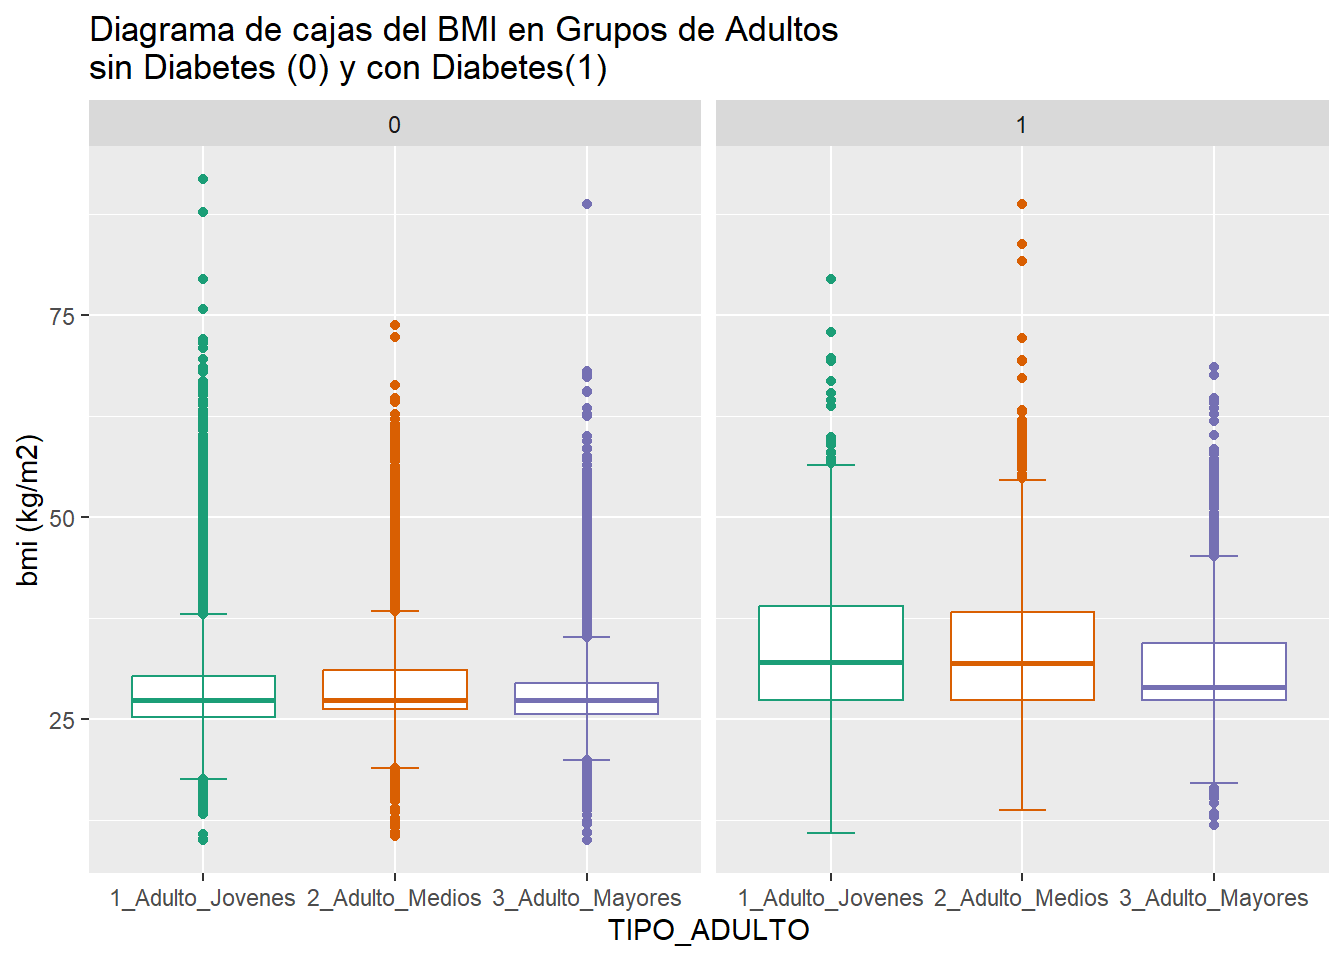
\includegraphics{Variables_files/figure-latex/unnamed-chunk-16-1.pdf}
\#\#\# \textbf{H. Analizando la variable HbA1c\_level - Hemoglobina
glicosidica:} \textbf{Comentario} Las medianas de los personas con
diabetes son mayores a las que no tienen la enfermedad . Para todos los
grupos de adultos.

\begin{Shaded}
\begin{Highlighting}[]
\DocumentationTok{\#\# Analizando la variable  HbA1c\_level  {-} Hemoglobina glicosidica}
\NormalTok{g }\OtherTok{\textless{}{-}}
  \FunctionTok{ggplot}\NormalTok{(diabetes\_Grupoadultos, }\FunctionTok{aes}\NormalTok{(}\AttributeTok{x =}\NormalTok{ TIPO\_ADULTO, }\AttributeTok{y =}\NormalTok{ HbA1c\_level,}
                   \AttributeTok{color =}\NormalTok{ TIPO\_ADULTO)) }\SpecialCharTok{+}
    \FunctionTok{labs}\NormalTok{(}\AttributeTok{x =} \StringTok{"TIPO\_ADULTO"}\NormalTok{, }\AttributeTok{y =} \StringTok{"HbA1c\_level \%"}\NormalTok{, }\AttributeTok{title =} \StringTok{"Diagrama de cajas del HbA1c\_level en Grupos de Adultos}\SpecialCharTok{\textbackslash{}n}\StringTok{sin Diabetes (0) y con Diabetes(1)"}\NormalTok{) }\SpecialCharTok{+}
    \FunctionTok{scale\_color\_brewer}\NormalTok{(}\AttributeTok{palette =} \StringTok{"Dark2"}\NormalTok{, }\AttributeTok{guide =} \StringTok{"none"}\NormalTok{)}

\NormalTok{g }\SpecialCharTok{+} \FunctionTok{geom\_boxplot}\NormalTok{() }\SpecialCharTok{+} \FunctionTok{stat\_boxplot}\NormalTok{(}\AttributeTok{geom =} \StringTok{"errorbar"}\NormalTok{,}
               \AttributeTok{width =} \FloatTok{0.25}\NormalTok{) }\SpecialCharTok{+} \FunctionTok{facet\_wrap}\NormalTok{(}\SpecialCharTok{\textasciitilde{}}\NormalTok{ diabetes)}
\end{Highlighting}
\end{Shaded}

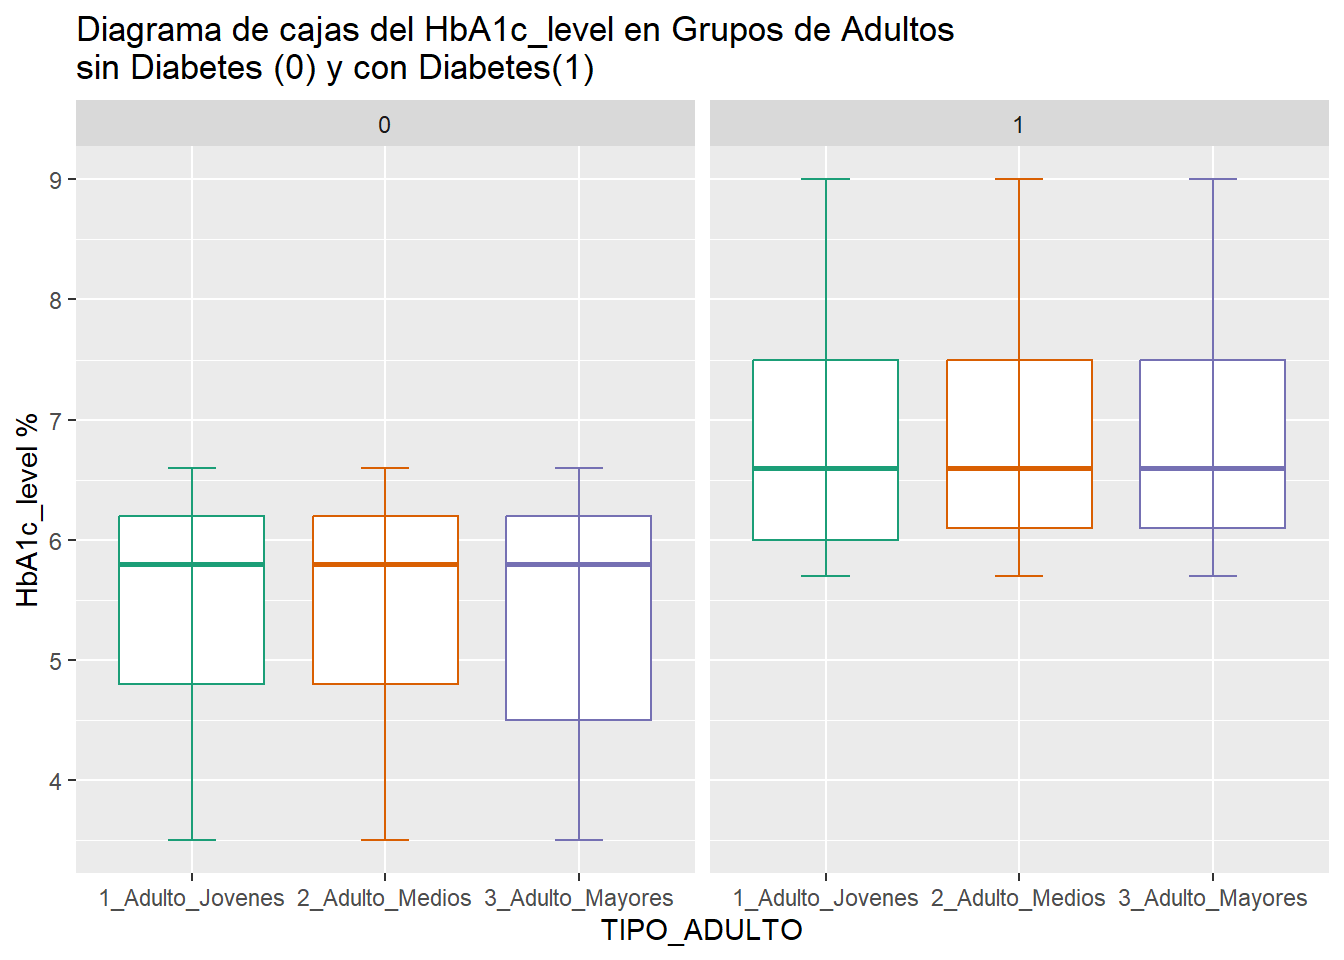
\includegraphics{Variables_files/figure-latex/unnamed-chunk-17-1.pdf}
\#\#\# \textbf{I. Analizando la variable Glucosa en sangre:}

\textbf{Comentario} Las medianas de los personas con diabetes son
mayores a las que no tienen la enfermedad . Para todos los grupos de
adultos.

\begin{Shaded}
\begin{Highlighting}[]
\DocumentationTok{\#\# Analizando la variable   Glucosa en sangre}
\NormalTok{g }\OtherTok{\textless{}{-}}
  \FunctionTok{ggplot}\NormalTok{(diabetes\_Grupoadultos, }\FunctionTok{aes}\NormalTok{(}\AttributeTok{x =}\NormalTok{ TIPO\_ADULTO, }\AttributeTok{y =}\NormalTok{ blood\_glucose\_level,}
                   \AttributeTok{color =}\NormalTok{ TIPO\_ADULTO)) }\SpecialCharTok{+}
    \FunctionTok{labs}\NormalTok{(}\AttributeTok{x =} \StringTok{"TIPO\_ADULTO"}\NormalTok{, }\AttributeTok{y =} \StringTok{"blood\_glucose\_level mg/dl"}\NormalTok{, }\AttributeTok{title =} \StringTok{"Diagrama de cajas del Glucosa en sangre en Grupos de Adultos}\SpecialCharTok{\textbackslash{}n}\StringTok{sin Diabetes (0) y con Diabetes(1)"}\NormalTok{) }\SpecialCharTok{+}
    \FunctionTok{scale\_color\_brewer}\NormalTok{(}\AttributeTok{palette =} \StringTok{"Dark2"}\NormalTok{, }\AttributeTok{guide =} \StringTok{"none"}\NormalTok{)}

\NormalTok{g }\SpecialCharTok{+} \FunctionTok{geom\_boxplot}\NormalTok{() }\SpecialCharTok{+} \FunctionTok{stat\_boxplot}\NormalTok{(}\AttributeTok{geom =} \StringTok{"errorbar"}\NormalTok{,}
               \AttributeTok{width =} \FloatTok{0.25}\NormalTok{) }\SpecialCharTok{+} \FunctionTok{facet\_wrap}\NormalTok{(}\SpecialCharTok{\textasciitilde{}}\NormalTok{ diabetes)}
\end{Highlighting}
\end{Shaded}

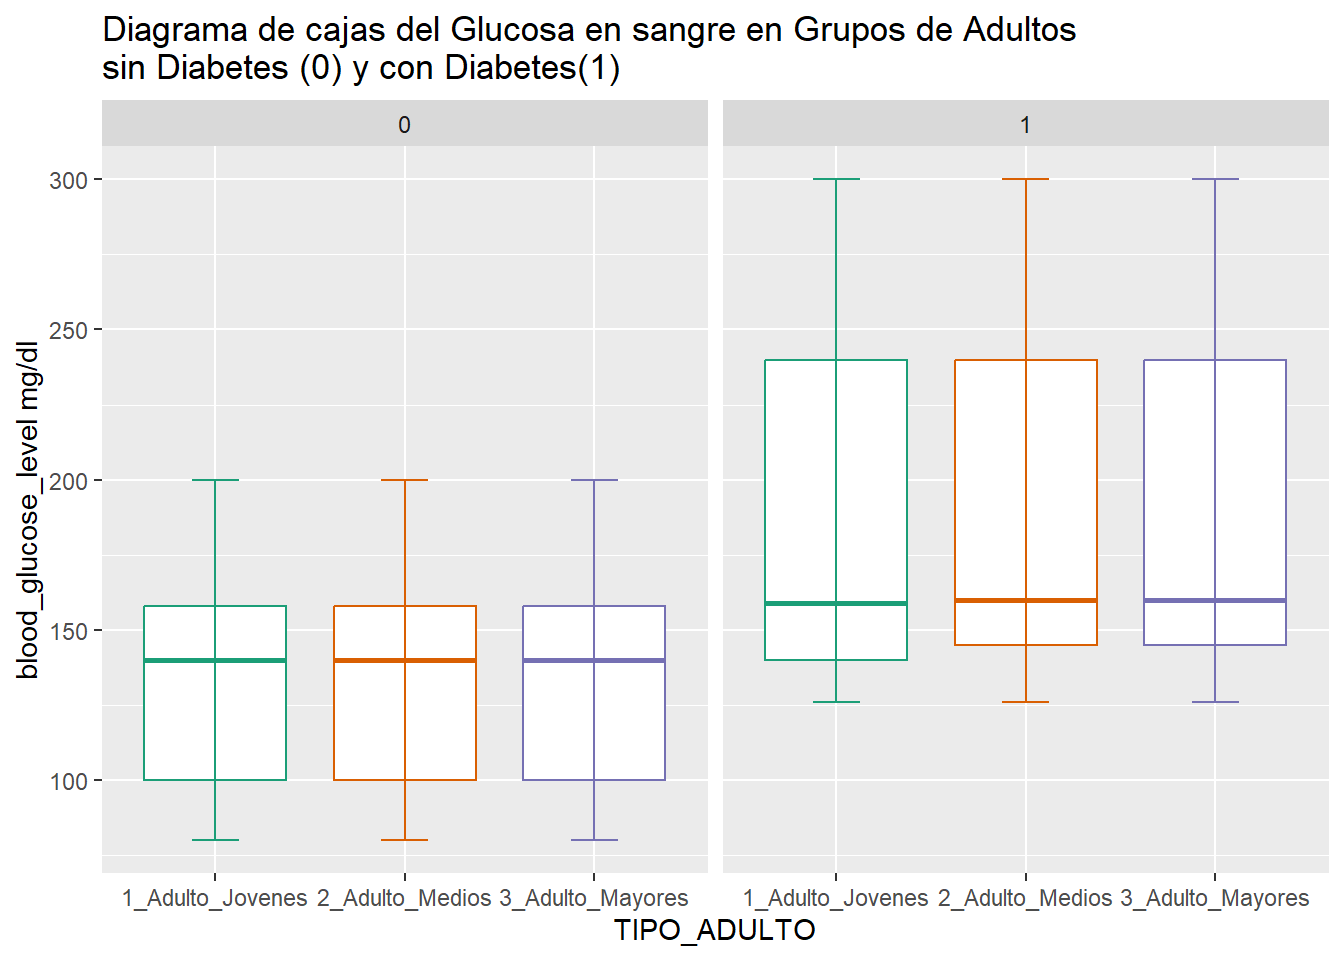
\includegraphics{Variables_files/figure-latex/unnamed-chunk-18-1.pdf}

\hypertarget{j.-prueba-de-correlacion-de-pearson}{%
\subsubsection{\texorpdfstring{\textbf{J. PRUEBA DE CORRELACION DE
PEARSON:}}{J. PRUEBA DE CORRELACION DE PEARSON:}}\label{j.-prueba-de-correlacion-de-pearson}}

Estamos usando Pearson porque todas las variables tienen una
\textbf{distribución bastante normal} 1

\begin{Shaded}
\begin{Highlighting}[]
\NormalTok{corm }\OtherTok{\textless{}{-}}
\NormalTok{  diabetes\_Grupoadultos }\SpecialCharTok{|\textgreater{}}
\NormalTok{  dplyr}\SpecialCharTok{::}\FunctionTok{select}\NormalTok{(bmi, blood\_glucose\_level, HbA1c\_level, age,heart\_disease,hypertension,diabetes) }\SpecialCharTok{|\textgreater{}}
\NormalTok{  corrr}\SpecialCharTok{::}\FunctionTok{correlate}\NormalTok{(}\AttributeTok{diagonal =} \DecValTok{1}\NormalTok{) }\SpecialCharTok{|\textgreater{}}
\NormalTok{  corrr}\SpecialCharTok{::}\FunctionTok{shave}\NormalTok{(}\AttributeTok{upper =} \ConstantTok{FALSE}\NormalTok{)}
\end{Highlighting}
\end{Shaded}

\begin{verbatim}
## Correlation computed with
## * Method: 'pearson'
## * Missing treated using: 'pairwise.complete.obs'
\end{verbatim}

\begin{Shaded}
\begin{Highlighting}[]
\NormalTok{corm}
\end{Highlighting}
\end{Shaded}

\begin{verbatim}
## # A tibble: 7 x 8
##   term                  bmi blood_glucose_level HbA1c_level     age heart_disease hypertension diabetes
##   <chr>               <dbl>               <dbl>       <dbl>   <dbl>         <dbl>        <dbl>    <dbl>
## 1 bmi                     1              0.0879      0.0796 -0.0229        0.0171       0.103     0.190
## 2 blood_glucose_level    NA              1           0.199   0.0983        0.0691       0.0816    0.455
## 3 HbA1c_level            NA             NA           1       0.0931        0.0682       0.0804    0.443
## 4 age                    NA             NA          NA       1             0.232        0.204     0.213
## 5 heart_disease          NA             NA          NA      NA             1            0.104     0.157
## 6 hypertension           NA             NA          NA      NA            NA            1         0.177
## 7 diabetes               NA             NA          NA      NA            NA           NA         1
\end{verbatim}

\begin{Shaded}
\begin{Highlighting}[]
\NormalTok{corm }\OtherTok{\textless{}{-}}
\NormalTok{  diabetes\_Grupoadultos }\SpecialCharTok{|\textgreater{}}
\NormalTok{  dplyr}\SpecialCharTok{::}\FunctionTok{select}\NormalTok{(bmi, blood\_glucose\_level, HbA1c\_level, age, heart\_disease, hypertension) }\SpecialCharTok{|\textgreater{}}
\NormalTok{  corrr}\SpecialCharTok{::}\FunctionTok{correlate}\NormalTok{(}\AttributeTok{diagonal =} \DecValTok{1}\NormalTok{) }\SpecialCharTok{|\textgreater{}}
\NormalTok{  corrr}\SpecialCharTok{::}\FunctionTok{shave}\NormalTok{(}\AttributeTok{upper =} \ConstantTok{FALSE}\NormalTok{)}
\end{Highlighting}
\end{Shaded}

\begin{verbatim}
## Correlation computed with
## * Method: 'pearson'
## * Missing treated using: 'pairwise.complete.obs'
\end{verbatim}

\begin{Shaded}
\begin{Highlighting}[]
\NormalTok{corm}
\end{Highlighting}
\end{Shaded}

\begin{verbatim}
## # A tibble: 6 x 7
##   term                  bmi blood_glucose_level HbA1c_level     age heart_disease hypertension
##   <chr>               <dbl>               <dbl>       <dbl>   <dbl>         <dbl>        <dbl>
## 1 bmi                     1              0.0879      0.0796 -0.0229        0.0171       0.103 
## 2 blood_glucose_level    NA              1           0.199   0.0983        0.0691       0.0816
## 3 HbA1c_level            NA             NA           1       0.0931        0.0682       0.0804
## 4 age                    NA             NA          NA       1             0.232        0.204 
## 5 heart_disease          NA             NA          NA      NA             1            0.104 
## 6 hypertension           NA             NA          NA      NA            NA            1
\end{verbatim}

\begin{Shaded}
\begin{Highlighting}[]
\NormalTok{corm }\OtherTok{\textless{}{-}}\NormalTok{ corm }\SpecialCharTok{|\textgreater{}}
\NormalTok{  tidyr}\SpecialCharTok{::}\FunctionTok{pivot\_longer}\NormalTok{(}
    \AttributeTok{cols =} \SpecialCharTok{{-}}\NormalTok{term,}
    \AttributeTok{names\_to =} \StringTok{"colname"}\NormalTok{,}
    \AttributeTok{values\_to =} \StringTok{"corr"}
\NormalTok{  ) }\SpecialCharTok{|\textgreater{}}
\NormalTok{  dplyr}\SpecialCharTok{::}\FunctionTok{mutate}\NormalTok{(}
    \AttributeTok{rowname =}\NormalTok{ forcats}\SpecialCharTok{::}\FunctionTok{fct\_inorder}\NormalTok{(term),}
    \AttributeTok{colname =}\NormalTok{ forcats}\SpecialCharTok{::}\FunctionTok{fct\_inorder}\NormalTok{(colname),}
    \AttributeTok{label =}\NormalTok{ dplyr}\SpecialCharTok{::}\FunctionTok{if\_else}\NormalTok{(}\FunctionTok{is.na}\NormalTok{(corr), }\StringTok{""}\NormalTok{, }\FunctionTok{sprintf}\NormalTok{(}\StringTok{"\%1.2f"}\NormalTok{, corr))}
\NormalTok{  )}
\end{Highlighting}
\end{Shaded}

\begin{Shaded}
\begin{Highlighting}[]
\FunctionTok{ggplot}\NormalTok{(corm, }\FunctionTok{aes}\NormalTok{(rowname, }\FunctionTok{fct\_rev}\NormalTok{(colname),}
                 \AttributeTok{fill =}\NormalTok{ corr)) }\SpecialCharTok{+}
  \FunctionTok{geom\_tile}\NormalTok{() }\SpecialCharTok{+}
  \FunctionTok{geom\_text}\NormalTok{(}\FunctionTok{aes}\NormalTok{(}
    \AttributeTok{label =}\NormalTok{ label,}
    \AttributeTok{color =} \FunctionTok{abs}\NormalTok{(corr) }\SpecialCharTok{\textless{}}\NormalTok{ .}\DecValTok{75}
\NormalTok{  )) }\SpecialCharTok{+}
  \FunctionTok{coord\_fixed}\NormalTok{(}\AttributeTok{expand =} \ConstantTok{FALSE}\NormalTok{) }\SpecialCharTok{+}
  \FunctionTok{scale\_color\_manual}\NormalTok{(}
    \AttributeTok{values =} \FunctionTok{c}\NormalTok{(}\StringTok{"white"}\NormalTok{, }\StringTok{"black"}\NormalTok{),}
    \AttributeTok{guide =} \StringTok{"none"}
\NormalTok{  ) }\SpecialCharTok{+}
  \FunctionTok{scale\_fill\_distiller}\NormalTok{(}
    \AttributeTok{palette =} \StringTok{"PuOr"}\NormalTok{, }\AttributeTok{na.value =} \StringTok{"white"}\NormalTok{,}
    \AttributeTok{direction =} \DecValTok{1}\NormalTok{, }\AttributeTok{limits =} \FunctionTok{c}\NormalTok{(}\SpecialCharTok{{-}}\DecValTok{1}\NormalTok{, }\DecValTok{1}\NormalTok{),}
    \AttributeTok{name =} \StringTok{"Pearson}\SpecialCharTok{\textbackslash{}n}\StringTok{Correlation:"}
\NormalTok{  ) }\SpecialCharTok{+}
  \FunctionTok{labs}\NormalTok{(}\AttributeTok{x =} \ConstantTok{NULL}\NormalTok{, }\AttributeTok{y =} \ConstantTok{NULL}\NormalTok{) }\SpecialCharTok{+}
  \FunctionTok{theme}\NormalTok{(}\AttributeTok{panel.border =} \FunctionTok{element\_rect}\NormalTok{(}\AttributeTok{color =} \ConstantTok{NA}\NormalTok{, }\AttributeTok{fill =} \ConstantTok{NA}\NormalTok{),}
        \AttributeTok{legend.position =} \FunctionTok{c}\NormalTok{(.}\DecValTok{85}\NormalTok{, .}\DecValTok{8}\NormalTok{))}
\end{Highlighting}
\end{Shaded}

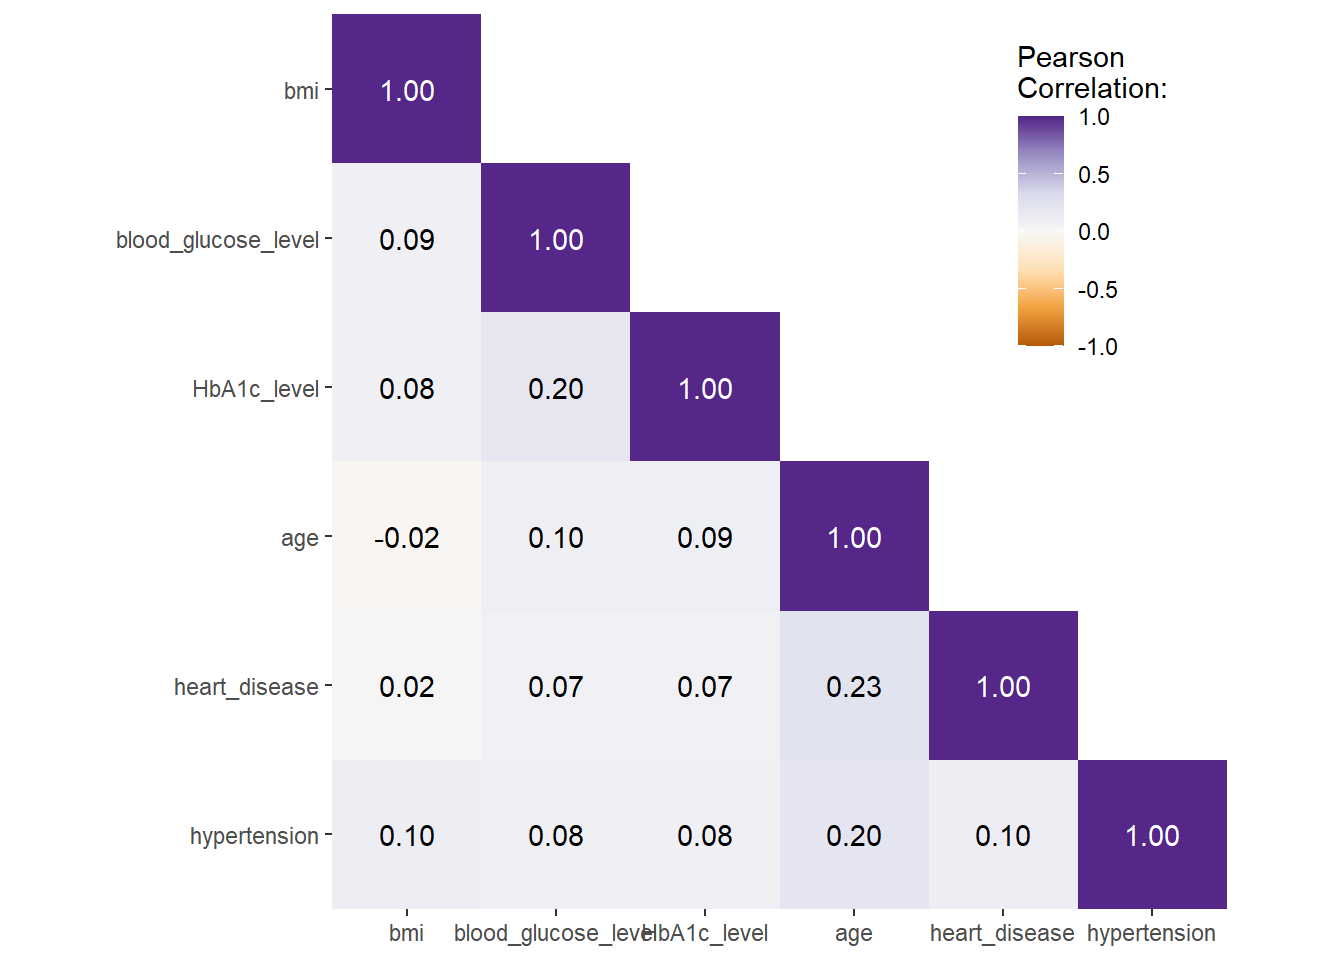
\includegraphics{Variables_files/figure-latex/unnamed-chunk-21-1.pdf}

\end{document}
